\documentclass[crop=false, class=memoir]{standalone}
\usepackage[utf8]{inputenc}%Nødvendig for danske bogstaver
\usepackage[danish]{babel}%Sørger for at ting LaTeX gør automatisk er på dansk
\usepackage{csquotes}
\usepackage{geometry}%Til opsætning af siden
\geometry{lmargin = 2.5cm,rmargin = 2.5cm}%sætter begge magner
\usepackage{lipsum}%Fyldtekst, til brug under test af layoutet
\usepackage{float}
\usepackage{graphicx}%Tillader grafik
\usepackage{epstopdf}%Tillader eps filer
\usepackage{marginnote}% Noter i margen
\interfootnotelinepenalty=10000 %undgår at fodnoter bliver spilittet op.
\usepackage[sorting=none]{biblatex}
\addbibresource{litteratur.bib}
\usepackage[hidelinks]{hyperref}%Tillader links
\usepackage{subcaption} % Tillader underfigurer
\usepackage[font={small,sl}]{caption}	% Caption med skrå tekst ikke kursiv

\usepackage{xcolor} %Bruges til farver
\usepackage{forloop} %Bruges til nemmere for loops

\newcounter{opgave}[chapter] %Definerer opgavenumrene og hvornår de nulstilles
\renewcommand{\theopgave}{\thechapter.\arabic{opgave}} %Definerer udseende af opgavenummereringen
\newcounter{delopgave}[opgave] %Definerer delopgavenumrene
\newcounter{lvl} %Definerer en "variabel" til senere brug

\definecolor{markerColor}{rgb}{0.0745098039, 0.262745098, 0.584313725} %Definerer farven af markøren
\newcommand{\markerSymbol}{\ensuremath{\bullet}} %Definerer tegnet for markøren
\newlength{\markerLength} %Definerer en ny længde
\settowidth{\markerLength}{\markerSymbol} %Sætter den nye længde til bredden af markøren

\newenvironment{opgave}[2][0]{%Definerer det nye enviroment, hvor sværhedsgraden er den første parameter med en default på 0
\newcommand{\opg}{\refstepcounter{delopgave}\par\vspace{0.1cm}\noindent\textbf{\thedelopgave)\space}}%Definerer kommando til delopgave
\refstepcounter{opgave}%Forøger opgavenummer med 1 og gør den mulig at referere til
\setcounter{lvl}{#1}%Sætter "variablen" lvl lig med angivelsen af sværhedsgraden
\noindent\hspace*{-0.75em}\hspace*{-\value{lvl}\markerLength}\forloop{lvl}{0}{\value{lvl}<#1}{{\color{markerColor}\markerSymbol}}\hspace*{0.75em}%Sætter et antal af markører svarende til sværhedsgraden
\textbf{Opgave \theopgave : #2}\newline\nopagebreak\ignorespaces}{\bigskip} %Angiver udseende af titlen på opgaverne samt mellemrummet mellem opgaver



\usepackage{mathtools}%Værktøjer til at skrive ligninger
\renewcommand{\phi}{\varphi}%Vi bruger varphi
\renewcommand{\epsilon}{\varepsilon}%Vi bruger varepsilon
\usepackage{physics}%En samling matematikmakroer til brug i fysiske ligninger
\usepackage{braket}%Simplere kommandoer til bra-ket-notation
\usepackage{siunitx}%Pakke der håndterer SI enheder godt
\DeclareSIUnit\clight{\text{\ensuremath{c}}} % Lysets fart i vakuum som c og ikke c_0
\usepackage{chemmacros}
\usechemmodule{isotopes}
\usepackage{tikz}
\usepackage[danish]{cleveref}
\usepackage{nicefrac}
% \renewcommand{\ref}[1]{\cref{#1}}
\creflabelformat{equation}{#2(#1)#3}
\crefrangelabelformat{equation}{#3(#1)#4 to #5(#2)#6}
\crefname{equation}{ligning}{ligningerne}
\Crefname{equation}{Ligning}{Ligningerne}
\crefname{section}{afsnit}{afsnitene}
\Crefname{section}{Afsnit}{Afsnitene}
\crefname{figure}{figur}{figurene}
\Crefname{figure}{Figur}{Figurene}
\crefname{table}{tabel}{tabellerne}
\Crefname{table}{Tabel}{Tabellerne}
\crefname{opgave}{opgave}{opgaverne}
\Crefname{opgave}{Opgave}{Opgaverne}
\crefname{delopgave}{delopgave}{delopgaverne}
\Crefname{delopgave}{Delopgave}{Delopgaverne}

\newcommand{\eqbox}[1]{\begin{empheq}[box=\fbox]{align}
	\begin{split}
	#1
	\end{split}
\end{empheq}}

\newcommand{\kb}{\ensuremath{k_\textsc{b}}}

\DeclareSIUnit{\parsec}{pc}
\DeclareSIUnit{\lightyear}{ly}
\DeclareSIUnit{\astronomicalunit}{AU}
\DeclareSIUnit{\year}{yr}
\DeclareSIUnit{\solarmass}{M_\odot}
\DeclareSIUnit{\solarradius}{R_\odot}
\DeclareSIUnit{\solarluminosity}{L_\odot}
\DeclareSIUnit{\solartemperature}{T_\odot}
\DeclareSIUnit{\earthmass}{M_\oplus}
\DeclareSIUnit{\earthradius}{R_\oplus}
\DeclareSIUnit{\jupitermass}{M_J}

% Infobokse og lignende
% http://mirrors.dotsrc.org/ctan/graphics/awesomebox/awesomebox.pdf
% \usepackage{awesomebox}


% Egen infobokse (virker kun med begrænsede symboler)

\usepackage[framemethod=tikz]{mdframed}
\usetikzlibrary{calc}
\usepackage{kantlipsum}

\usepackage[tikz]{bclogo}

\tikzset{
    % lampsymbol/.style={scale=2,overlay}
    % lampsymbol/.pic={\centering\tikz[scale=5]\node[scale=10,rotate=30]{\bclampe}}.style={scale=2,overlay}
    infosymbol/.style={scale=2,overlay}
}

\newmdenv[
    hidealllines=true,
    nobreak,
    middlelinewidth=.8pt,
    backgroundcolor=blue!10,
    frametitlefont=\bfseries,
    leftmargin=.3cm, rightmargin=.3cm, innerleftmargin=2cm,
    roundcorner=5pt,
    % skipabove=\topsep,skipbelow=\topsep,
    singleextra={\path let \p1=(P), \p2=(O) in ($(\x2,0)+0.92*(1.1,\y1)$) node[infosymbol] {\bcinfo};},
    % singleextra={\path let \p1=(P), \p2=(O) in ($(\x2,0)+0.5*(2,\y1)$) node[infosymbol] {\bcinfo};},
]{info}

% Skal bruges som
% \begin{info}[frametitle={Titel}]
%     Tekst
% \end{info}
\usepackage{import}
\begin{document}
\chapter{Kosmologi} \label{chap:kosmo_opg}

\begin{opgave}[1]{Hubbleloven}
    \opg Forklar hvorfor Hubbleloven kun gælder hvis $v>0$.
    \opg Kan Hubbleloven bruges til at bestemme afstande til himmellegemer, hvis lys er er blåforskudt?
\end{opgave}

\begin{opgave}[1]{Den kritiske tæthed}
Den kritiske tæthed, $\rho_c$, kan defineres ud fra Friedmannligningen som den værdi af $\rho$, der opfylder ligningen for et fladt univers.
\opg Hvilken værdi har $\kappa$ i et fladt univers?
\opg Vis at den kritiske tæthed er
%
\begin{align}
    \rho_c = \frac{1}{8\pi G}\left(3H^2 - \Lambda\right).
\end{align}
%
\opg Argumenter for at hvis $\Lambda \ll 3H^2$ så er
%
\begin{align} \label{eq:rho_c}
    \rho_c \simeq \frac{3H^2}{8\pi G}.
\end{align}
%
\opg Brug ligning \eqref{eq:rho_c} til at vise at den kritiske tæthed i Universet med den nuværende værdi af Hubbleparameteren, $H_0$, er
%
\begin{align*}
    \rho_\textup{c} = \SI{8.6e-27}{\kilo\gram\per\cubic\metre}.
\end{align*}
\end{opgave}



\begin{opgave}[2]{Dopplerforskydning}%{2}
	Formlen for frekvensen ved Dopplerforskydning er
	\begin{align}
		f_\textup{obs} = \frac{c+v_\textup{obs}}{c+v_\textup{kilde}} f_\textup{kilde},
	\end{align}
	hvor $c$ er lydens hastighed i mediet, $f_\textup{obs}$ er den observerede frekvens (udefra), $f_\textup{kilde}$ er den udsendte frekvens, $v_\textup{obs}$ er observatørens hastighed og $v_\textup{kilde}$ er kildens hastighed.
	\opg En politibil kører mod dig 30 meter væk, men er 20 meter fra centrum af vejen når du kigger ligeud (se skitsen på \cref{politi}). Tegn hastighedsvektoren og hastighedskomponenterne der peger henholdsvis parallelt med din synsvinkel og vinkelret på den. 
	\opg Bilens speedometer viser, at den kører \SI{50}{\km\per\hour}. Brug trigonometri til at beregne hvor stor en hastighedskomponent, der peger mod dig (radiel hastighed). Skitsér groft en graf over radiel hastighed som funktion af tid og antag, at bilens hastighed er konstant.
	\opg Politibilens sirene udsender lyd med en frekvens på \SI{800}{\hertz}. Du står stille, og det er en let kølig dag med 15 grader, hvor lydens fart i luft er \SI{340}{\metre\per\second}. Ved hvilken frekvens hører du tonen?
	\begin{figure}[]
		\centering
		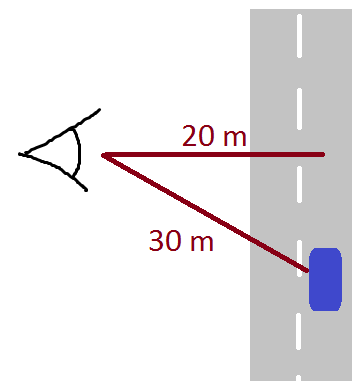
\includegraphics[width=0.5\textwidth]{Kosmo/kosmofig/Politi.png}
		\caption{}
		\label{politi}
	\end{figure}
\end{opgave}

\begin{opgave}[1]{Skalafaktor}%{1}
	Temperaturen af den kosmiske mikrobølgebaggrund er i dag \SI{2.73}{\kelvin}. Strålingen blev udsendt ved ``rekombinationen'', hvor universet var koldt nok til at elektroner kunne binde sig til atomerne. Det var en mindre exciteret tilstand, så atomerne udsendte energi som fotoner. Man kan måle, at det har krævet en temperatur på kun \SI{3000}{\kelvin}. Brug at temperaturen udviklede sig som
	\begin{align}
		T(t)=\frac{T_0}{a(t)}
	\end{align}
	til at finde ud af, ved hvilken rødforskydning rekombinationen fandt sted.
\end{opgave}

\begin{opgave}[1]{Rødforskydning af kvasar}%{1}
	Kvasarer (eng: ``quasars'' fra ``quasi-stellar radio sources'') er de mest energirige og
	fjerne medlemmer af objekterne kendt som aktive galaksekerner (eng: ``AGN: Active
	Galactic Nuclei''). Kvasarer har siden deres opdagelse været omgivet af mystik, men
	der er nu opnået generel enighed om, at de er kompakte regioner i massive galakser,
	der indeholder det centrale supermassive sorte hul. De kæmpe mængder energi der
	bliver udstrålet af kvasarerne stammer fra al stoffet, som falder ind mod det sorte
	hul og bliver slynget ud.
	Et kvasar-spektrum er vist i \cref{kvasar}.
	\\
	I Balmer-serien hopper en elektron til 2. orbital fra en mere exciteret tilstand. Den første af disse kaldes H-$\alpha$ og er faldet fra orbital 3 til 2. Den næste er H-$\beta$ fra orbital 4 til 2 osv. Fotoner, der udsendes ved H-$\alpha$-overgangen, har en bølgelængde på \SI{656}{\nano\meter}. Ofte måler man i Ångstrøm (\si{\angstrom}) som er \SI{e-10}{\metre}.\\
	%Aflæs bølgelængden for H-$\beta$ på Figur \ref{spektrum} og beregn rødforskydningen.
		\begin{figure}[]
			\centering
			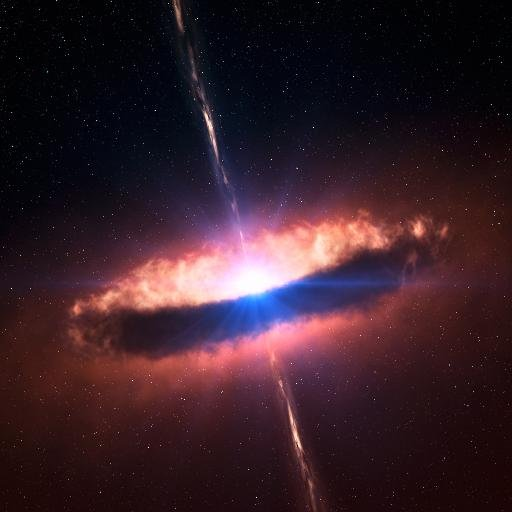
\includegraphics[width=0.5\textwidth]{Kosmo/kosmofig/kvasarkunst.jpg}
			\caption{En kunstnerisk forestilling af en kvasar. Kilde: \cite{NASA_ESA_quasar}} %https://pbs.twimg.com/profile_images/683524276058763264/xyAc-NvD.jpg
			\label{kvasarkunst}
		\end{figure}
	\begin{figure}[]
		\centering
		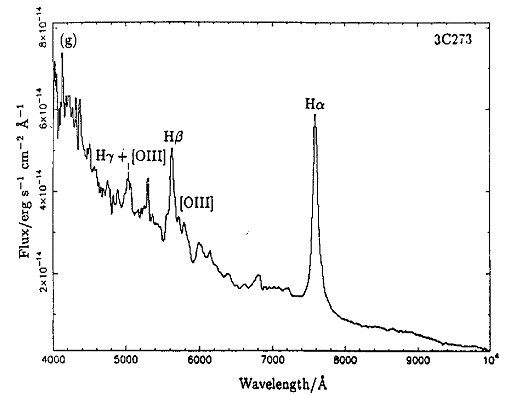
\includegraphics[width=0.6\textwidth]{Kosmo/kosmofig/kvasar.png}
		\caption{Spektrum af kvasaren 3C273. Kilde: \cite{YatesGardenQuasarSpectrum}} %http://www.astrosurf.com/buil/us/spe6/qso1.gif
		\label{kvasar}
	\end{figure}
	\opg Ud fra din viden om H-$\alpha$-overgangen, bevæger kvasaren sig så mod eller væk fra os?
	\opg Hvad er kvasarens radielle hastighed?
	\opg Man ser tit, at spektrallinjerne fra kvasarer er meget brede, fordi gassen bevæger sig hurtigt omkring det sorte hul, hvilket giver en Doppler-forbredning
	(lyset bliver både rød- og blåforskudt). Estimér bredden af H-$\alpha$-linjen, $\Delta\lambda_\textup{obs}$, og udregn gassens fart ved 
	\begin{align}
		v_\textup{gas}=\frac{\Delta \lambda_\textup{obs}}{2\lambda_{0}}c
	\end{align}
\end{opgave}

\begin{opgave}[3]{Afstande} %{3}
	\\  		
	\begin{figure}[]
			\centering
			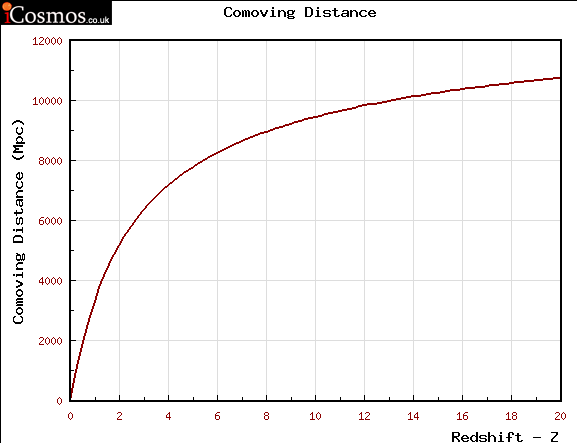
\includegraphics[width=0.5\textwidth]{Kosmo/kosmofig/ComovingDistance.png}
			\caption{Kilde: \cite{vardanyanICosmosCosmologyCalculator}.} %http://www.icosmos.co.uk/index.html
			\label{comoving} 
		\end{figure}
	\opg Opskriv luminositetsafstanden $d_L$ som funktion af vinkelafstanden $d_A$.
	\opg I et fladt univers er $d_M = d_C$. $d_C$ kaldes comoving distance, og med $\Omega_m = \num{0.3}$ og $\Omega_{\Lambda} = \num{0.7}$ opfører det sig som plottet på \cref{comoving}. 
	Hvor stor er $d_L$ og $d_A$ ved $z = 1$? \\
	Hvad med ved $z = 9$? Giver ændringerne mening?
	\opg Hvor stor er den radielle hastighed for et objekt med $z = 10$? Oplys svaret som procent af lysets fart i vakuum. Dengang var universet for resten kun  478 mio. år gammelt.
\end{opgave}

\begin{opgave}[1]{Andromeda-galaksen}
		\begin{figure}[]
			\centering
			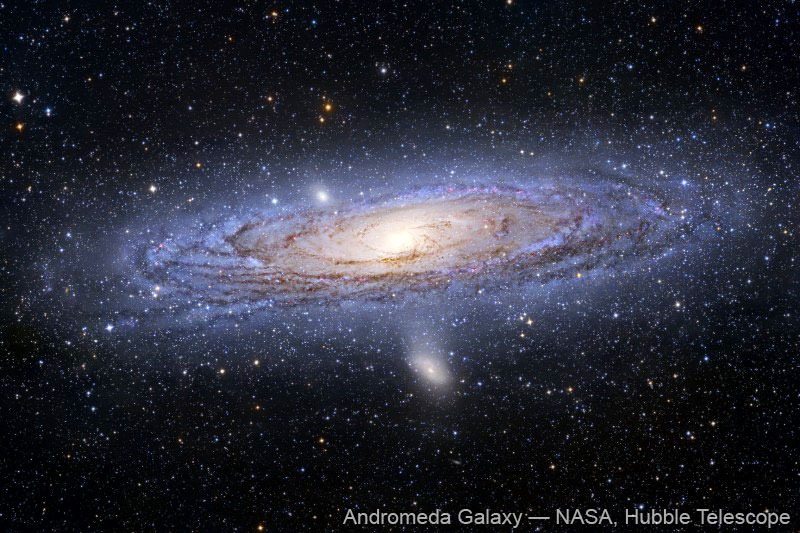
\includegraphics[width=0.5\textwidth]{Kosmo/kosmofig/andromeda.jpg}
			\caption{Kilde: \cite{AndromedaGalaxy2019}.} %https://upload.wikimedia.org/wikipedia/commons/9/98/Andromeda_Galaxy_%28with_h-alpha%29.jpg
			\label{andromeda} 
		\end{figure}
	Andromeda-galaksen eller Messier-31 (M31) er den nærmeste spiralgalakse, og den største galakse i den Lokale Gruppe, som er en samling af ca. 50 galakser, heriblandt vores egen, Mælkevejen.  
	\opg Det observerede lys fra Andromeda har en rødforskyning på $z = -0.001$.
	%\opg Det observerede lys fra Andromeda har en rødforskydning på $z = −0.001$.
	Hvad er Hubbleafstanden til galaksen, fundet ved hjælp af Hubbles lov? Antag Hubblekonstanten er $H_0 = \SI{70}{\km\per\second\per\mega\parsec}$.
	\opg Gennem andre metoder har man fundet afstanden til 2,5 mio. lysår. Hvornår støder Andromeda og Mælkevejen sammen? Hvad tror du, det kommer til at betyde? Antag hastigheden er konstant, og Andromeda har direkte kurs mod os.
\end{opgave}

\begin{opgave}[3]{Et univers af bolde}
Massetætheden i et univers kun bestående af bolde med massen $m_\textup{b} = \SI{1}{M_\odot}$ (én solmasse) er
%
\begin{align} \label{eq:antalsdensitet}
    \rho = n_\textup{b}m_\textup{b},
\end{align}
%
hvor $n_\textup{b}$ er antalstætheden af bolde -- det vil sige antallet af bolde per volumen.
\opg Hvad skal antalstætheden af bolde være for at universet har den nuværende kritiske tæthed $\rho_\textup{c} = \SI{8.6e-27}{\kilogram\per\cubic\metre}$?
\opg Den gennemsnitlige afstand mellem bolde i et sådant univers skalerer med antalstætheden, og det kan beskrives ved $d_\textup{b} = n_\textup{b}^{-1/3}$. Bestem denne afstand.
\opg Afstanden til den fjerneste galakse vi kender er $d_\textup{max} \approx \SI{9.8}{\giga\parsec}$. %Bestem $d_\textup{max}/d_\textup{b}$.
Den gennemsnitlige afstand lys kan rejse før det støder på en bold er
\begin{align}
	d_\textup{MFP} = (A n)^{-1}
\end{align}
hvor $A$ er boldenes tværsnitsareal. MFP står for mean free path. Lad os sige hver bold har radius $R_\odot$. Beregn $d_\textup{MFP}$ i parsec, og bestem $d_\textup{max}/d_\textup{MFP}$.

\opg Sandsynligheden for en foton rammer en bold stiger, des længere den rejser (hvis vi ser bort fra udvidelsen). Sandsynligheden for ikke at ramme en bold inden afstand $x$ er
\begin{align}
	P(x) = e^{-x/d_\textup{MFP}}.
\end{align}
Virker det sandsynligt at kunne se noget på den afstand vi kan, hvis vi levede i et univers af sådanne bolde?

\opg Opskriv et samlet udtryk for sandsynligheden for at se ud til afstand $x$ hvori massen af boldene indgår. Vil en større masse af boldene øge eller mindske sigtbarheden? Hvad med radius? 

Uden at behøve at regne på det, kan du se hvad der ville ske hvis vi fordoblede både masse og radius?

\opg Ville vi kunne se til $d_\textup{max}$ hvis universet bestod af balloner på \SI{20}{\cm} og \SI{5}{\gram}? Hvad fortæller det os om fordelingen af masse i universet og de antagelser vi har gjort os?

Du kan også for sjov indsætte din egen radius og masse.

%\opg
%Havde man brugt Mælkevejens masse, $m_\textup{b} = \SI{1e12}{M_\odot}$, ville man få $d_\textup{max}/d_\textup{b} = \SI{2.2e3}{}$, mens massen for en typisk galaksehob, $m_\textup{b} = \SI{1e15}{M_\odot}$, giver $d_\textup{max}/d_\textup{b} = \SI{2.2e2}{}$. Hvad fortæller disse udregninger os om Universet?
\end{opgave}

\begin{opgave}[4]{Fra stråling til stof}
I kompendiets \cref{k-kosmo:fig:figDensity} ser man at forskellige af universets komponenter har domineret universet på forskellige tidspunkter. 

\opg Hvad betyder det at en komponent \emph{dominerer}? \\

Hvis én komponent dominerer i én periode af universet, og en anden på et senere tidspunkt, er der sket en overgang i fordelingen af energi i universet.

\opg Overvej hvad der sker med komponenternes densiteter under denne overgang

\opg Brug \cref{k-kosmo:eq:omega} og \cref{k-kosmo:eq:densities} i kompendiet til at bestemme densiteten for stråling og stof i dag, $\rho_{\textup{R},0}$ og $\rho_{\textup{m},0}$ - Husk at $\rho_\textup{c} = \SI{8,6e-27}{\kilogram \per \cubic \meter}$.

\opg Ved hvilken rødforskydning gik universet fra at være domineret af stråling til at være domineret af stof? Hint: Hvad skal ${\rho_\textup{m}}/{\rho_\textup{R}}$ være ved overgangen?

\end{opgave}

\begin{opgave}[2]{Comahoben}
Galaksehobe er nogle af de største strukturer i universet. Helt basalt består de blot af en samling galakser, samt det løse gas og støv. Omkring $\SI{100}{\mega \parsec}$ fra Jorden ligger Comahoben, som indeholder $\sim\num{1000}$ galakser. 
%
Comahoben har en luminositet på $L = \SI{3e13}{\solarluminosity}$, hvor $\SI{1}{\solarluminosity} = \SI{3,828e26}{\watt}$ er Solens luminositet. 

\opg Hvor meget vejer Comahoben, hvis der er én solmasse per solluminositet? Brug her at Solens masse er $\SI{1}{\solarmass} = \SI{2e30}{\kilogram}$. \\

\indent Din ven kommer nu hen til dig. Hun fortæller dig, at hun har målt omdrejningshastigheden af en galakse i udkanten af Comahoben til $v = \SI{2,38e3}{\kilo \meter \per \second}$. Yderligere fortæller hun, at afstanden fra galaksen til Comahobens centrum er $\SI{12,5e6}{\lightyear}$.

\opg Hvad er massen af Comahoben baseret på hastigheden af denne galakse? Angiv gerne dit svar både i kilogram og solmasser.

\opg Hvorfor er de to svar forskellige?

\end{opgave}

% \begin{opgave}[2]{Noget med magnituder}


% \end{opgave}

\end{document}